\subsection{中断功能硬布线控制器}
\subsubsection{\tec 中断功能探究}
通过查阅\tec 实验指导书,得知\tec 模型计算机中有一个简单的单级中断,支持单级中断、
单个中断请求, 有中断屏蔽功能。
\par
\tec 模型计算机中有2条指令用于允许和屏蔽中断。DI指令称作关中断指令。词条指令执行后,
即使发生 中断请求,\tec 也不响应中断请求。EI指令称作开中断指令,此条指令执行后,
\tec 响应中断。 在时序发生器中,设置了一个允许中断触发器EN\_INT,当它为1时,
允许中断; 当它为0时,禁止中断发生。 复位脉冲CLR\#使EN\_INT复位为0。
\begin{figure}[htbp]
    \label{tec8graph}
    \includegraphics[width=\textwidth]{figures/chapter3/tec8.png}
    \caption{\tec 模型计算机框图}
\end{figure}
然而,\tec 此次并没有提供IABUS、IAR和INTEN等信号,因此无法访问IAR寄存器来借助
板载功能实现中断。
\subsubsection{中断功能实现思路}
但是,在经过组内成员思考和讨论后,发现可以通过借用一个通用寄存器来作为PC的镜像的方式,
间接实现中断功能。在正常执行的时候,让R3的值在PCINC, PCADD和LPC等信号存在时同步变化,
进入中断后,停止R3值变化;读到IRET指令后,将R3的值恢复到PC中,实现中断返回。
\subsubsection{中断功能详细设计}
为实现中断功能,我们在之前设计的8位机器指令\footnote{ 由IR7\wave IR4+SWC+
    SWB+SWA+ST0 共8位组成} 的基础上在末尾增加一位ST1,扩充为9位机器指令。此外,
使用了控制台的PULSE信号,并增加了新信号如下。
\begin{table}[h]
    \centering
    \label{interrupt_signal}
    \begin{tabular}[c]{r | l }
        \hline
        变量      & 含义           \\
        \hline
        int0    & 中断标志位        \\
        en\_int & 中断允许标志位      \\ % \cline{2-2}
        inten   & 中断使能标志位      \\
        intdi   & 中断屏蔽标志位      \\
        st1     & 中断执行周期标志位    \\
        pulse   & 控制台pulse中断信号 \\
        \hline
    \end{tabular}
    \caption{中断各新增标志位的说明}
\end{table}
\begin{itemize}
    \item[$\diamond$ \textbf{int0}] 中断标志位,当传入pulse信号且en\_{}int为1时置1,
        进入中断阶段。
    \item[$\diamond$ \textbf{en\_int}] 中断允许标志位,在t3下降沿时,
        (inten | (en\_int \& !intdi))为1时则en\_int为1,即此时允许中断。
        为0时en\_int为0,表示此时禁止中断。
    \item[$\diamond$ \textbf{inten}] 中断使能标志位,仅当执行中断返回指令iret且节拍电位为
        w2时此标志位为1,表示离开中断子程序,\tec 再次能够进行中断。
    \item[$\diamond$ \textbf{intdi}] 中断屏蔽标志位,仅当中断执行周期标志位st1 == 1且
        节拍电位为w1时为1,表示进入中断服务程序,\tec 不能再进行中断。
    \item[$\diamond$ \textbf{st1}] 中断执行周期标志位,为1时进入中断处理程序,为0表示
        离开中断处理程序。
    \item[$\diamond$ \textbf{pulse}] \tec 的pulse信号,是按下pulse按钮产生的高电平有效
        的中断请求脉冲信号。
\end{itemize}
\begin{figure}[htbp]
    \centering
    \label{interrupt_control_flow}
    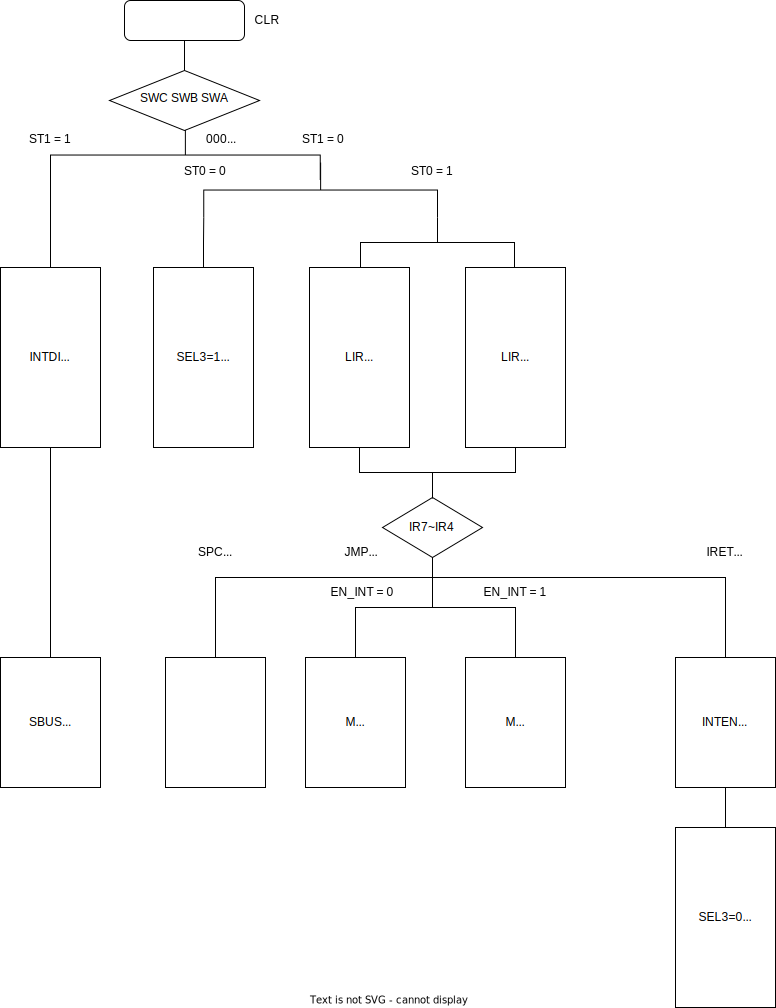
\includegraphics[width=\textwidth]{figures/chapter3/interrupt_control_flow.drawio.png}
    \caption{中断处理控制流程图}
\end{figure}
为了实现中断功能,对其他部分指令进行了改动。
\begin{itemize}
    \item 新增IRET指令如表\ref{interrupt_instruction_table},用于中断服务程序返回,在它的W2阶段开中断,W3阶段将R3的值
          赋给PC。
    \item 因为R3作为了PC的镜像,服务于中断返回,所以对其他指令屏蔽R3。
    \item 对JMP指令,由于在将寄存器的值赋给PC之外还要同步赋给R3,所以对JMP指令的格式
          和微指令进行改动如表\ref{interrupt_instruction_table}。
    \item 由于JC和JZ指令的低四位表示offset,占用了表示R3的位,导致无法让R3与PC
          同步变化。经过考虑后,认为可以通过增加新标志位st2,在st2 = 1的时候从存储器
          左端口读出offset到数据总线,再加到R3的值实现,并恢复st2 = 0。但是由于时间限制,
          没能成功实现。
\end{itemize}
\begin{table}[h]
    \centering
    \label{interrupt_instruction_table}
    \begin{tabular}[c]{|c|c|c|c|c|c|}
        \hline
        \multirow{2}*{名称} & \multirow{2}*{助记符} & \multirow{2}*{功能} & \multicolumn{3}{c|}{指令格式}                               \\ \cline{4-6}
        ~                 & ~                  & ~                 & IR7\wave IR4              & IR3\wave IR2 & IR1\wave IR0 \\
        \hline
        中断返回              & IRET               & $PC\leftarrow R3$ & 1111                      & XX           & XX           \\
        \hline
        无条件跳转             & JMP                & $PC\leftarrow Rd$ & 1001                      & 11           & Rd           \\
        \hline
    \end{tabular}
    \caption{为实现中断对指令的改动}
\end{table}
\subsubsection{中断处理流程}
中断处理的流程如图\ref{interrupt_control_flow}所示。
\begin{itemize}
    \item[$\diamond$ \textbf{R3作为PC的镜像}] 在中断允许标志位EN\_INT为1时,R3和PC保持同步变化。
        在取指令的时候,R3随PCINC同步自增。当JMP指令执行的时候,由于IR3\wave IR2已经规定为11,所以DRW
        置1即可同步将寄存器的值写入R3。
    \item[$\diamond$ \textbf{中断处理}] 按下CLR后,中断允许标志位en\_int置1,此时可以接受pulse
        信号使int0置1,从而进入中断。在每一个t3的下降沿,根据目前intdi和inten的状态来设置en\_int的值;对于intdi,只在st1 == 1且w1
        时期置1,inten只在IRET指令且w2周期时置1。因此,在IRET的w3时期就可以继续接受中断请求。此外,
        在双周期指令的w2和三周期指令的w3阶段,如果int0为1,则置st1 = 1,进入中断处理周期。
        \par
        在中断处理周期的w1,中断屏蔽位intdi置1,stop置1暂停程序,在t3下降沿置en\_int为0,int0为0。
        在w2的t3下降沿中写入PC的值时,置st1位0,标识中断处理周期结束,进入中断子程序。
        \par
        在中断子程序中,en\_int为0,R3将不与PC同步变化,直到读到IRET指令,在w2时期置inten为1,使en\_int
        在t3下降沿置1,标识可以再次进入中断。在w3时期将R3保存的进入中断时PC值赋给PC,退出中断,
        恢复断点,中断处理结束。
\end{itemize}
\subsubsection{多级中断实现思路}
为了实现多级中断功能,我们需要更多的存储空间用于存放中断服务程序的pc值,由于寄存器数量有限且使用频繁,我们决定使用存储器空间用于存放pc值。但是这样会存在一个问题,若需要实时同步存储器和PC寄存器的值,就需要能够实时获取存有当前执行程序pc值的存储器地址。因此,我们考虑仅使用一个寄存器作为栈顶指针寄存器存储该地址。
\par
具体实现方式即为执行程序过程中实时同步当前pc值和栈顶指针寄存器指向的存储器值,在接受到中断请求后,栈顶指针加一,指向新的存储器位置用于存放新的中断服务程序pc值。若预留足够的存储器空间,便可实现自定义级数的中断。不过由于时间不够充裕,我们并未实现该功能,现仅提供实现思路。